\chapter{動作検証}
\label{chp:tex_pro}
この章では動作検証の結果をスクリーンショットとソースコードを元に紹介する.
今回はGoogle Chrome上で動作させるため,他のWebブラウザ上ではUIが異なっている可能性がある.

\section{社員が写真を提出する}
\label{sec:tex_pro_cmd}
社員ページに顔写真提出するためのフォームを作成した.写真提出ボタンから提出する写真を選択し,
提出する.その実行しているスクリーンショットを図4.1,図4.2,図4.3,図4.4に示す.
face-api.jsを用いて,表情を分析し,それらの値と笑顔の値などに応じて加算される笑みポイントを
useStateで保存する(ソースコード4.1).
\\

\renewcommand{\lstlistingname}{ソースコード}

\begin{lstlisting}[caption=表情分析]
  const handleImage = async () => {
    const detections = await faceapi
      .detectAllFaces(imgRef.current, new faceapi.TinyFaceDetectorOptions())
      .withFaceExpressions();

    if (detections[0].expressions.happy >= 0.7) {
      setObject({
        expressions: {
          angry: detections[0].expressions.angry,
          disgusted: detections[0].expressions.disgusted,
          fearful: detections[0].expressions.fearful,
          happy: detections[0].expressions.happy,
          neutral: detections[0].expressions.neutral,
          sad: detections[0].expressions.sad,
          surprised: detections[0].expressions.surprised,
        },
        point: 3,
      });
    } else if (
      detections[0].expressions.happy >= 0.5 ||
      detections[0].expressions.surprised >= 0.7 ||
      detections[0].expressions.neutral >= 0.7
    ) {
      setObject({
        expressions: {
          angry: detections[0].expressions.angry,
          disgusted: detections[0].expressions.disgusted,
          fearful: detections[0].expressions.fearful,
          happy: detections[0].expressions.happy,
          neutral: detections[0].expressions.neutral,
          sad: detections[0].expressions.sad,
          surprised: detections[0].expressions.surprised,
        },
        point: 2,
      });
    } else if (
      detections[0].expressions.happy >= 0.3 ||
      detections[0].expressions.surprised >= 0.5 ||
      detections[0].expressions.neutral >= 0.5
    ) {
      setObject({
        expressions: {
          angry: detections[0].expressions.angry,
          disgusted: detections[0].expressions.disgusted,
          fearful: detections[0].expressions.fearful,
          happy: detections[0].expressions.happy,
          neutral: detections[0].expressions.neutral,
          sad: detections[0].expressions.sad,
          surprised: detections[0].expressions.surprised,
        },
        point: 1,
      });
    } else {
      setObject({
        expressions: {
          angry: detections[0].expressions.angry,
          disgusted: detections[0].expressions.disgusted,
          fearful: detections[0].expressions.fearful,
          happy: detections[0].expressions.happy,
          neutral: detections[0].expressions.neutral,
          sad: detections[0].expressions.sad,
          surprised: detections[0].expressions.surprised,
        },
        point: 0,
      });
    }
  };

  useEffect(() => {
    const loadModels = () => {
      Promise.all([
        faceapi.nets.tinyFaceDetector.loadFromUri("/models"),
        faceapi.nets.faceLandmark68Net.loadFromUri("/models"),
        faceapi.nets.faceExpressionNet.loadFromUri("/models"),
      ])
        .then(handleImage)
        .catch((e) => console.log(e));
    };

    imgRef.current && loadModels();
  }, []);
\end{lstlisting}

もし顔認識できない写真であれば,もう一度写真を提出させる処理をすることでエラー回避している
(ソースコード4.2).そのスクリーンショットを図4.5に示す.

\begin{lstlisting}[caption=顔認識エラー処理]
  if (object.length !== undefined) {
    return (
      <div>
        <p>顔認識できません。</p>
        <p
          className="submit reset"
          onClick={() => {
            setNum(1);
          }}
        >
          やり直す
        </p>
      </div>
    );
  }
\end{lstlisting}

\vspace{4mm}

\begin{figure}[!h]
	\begin{center}
			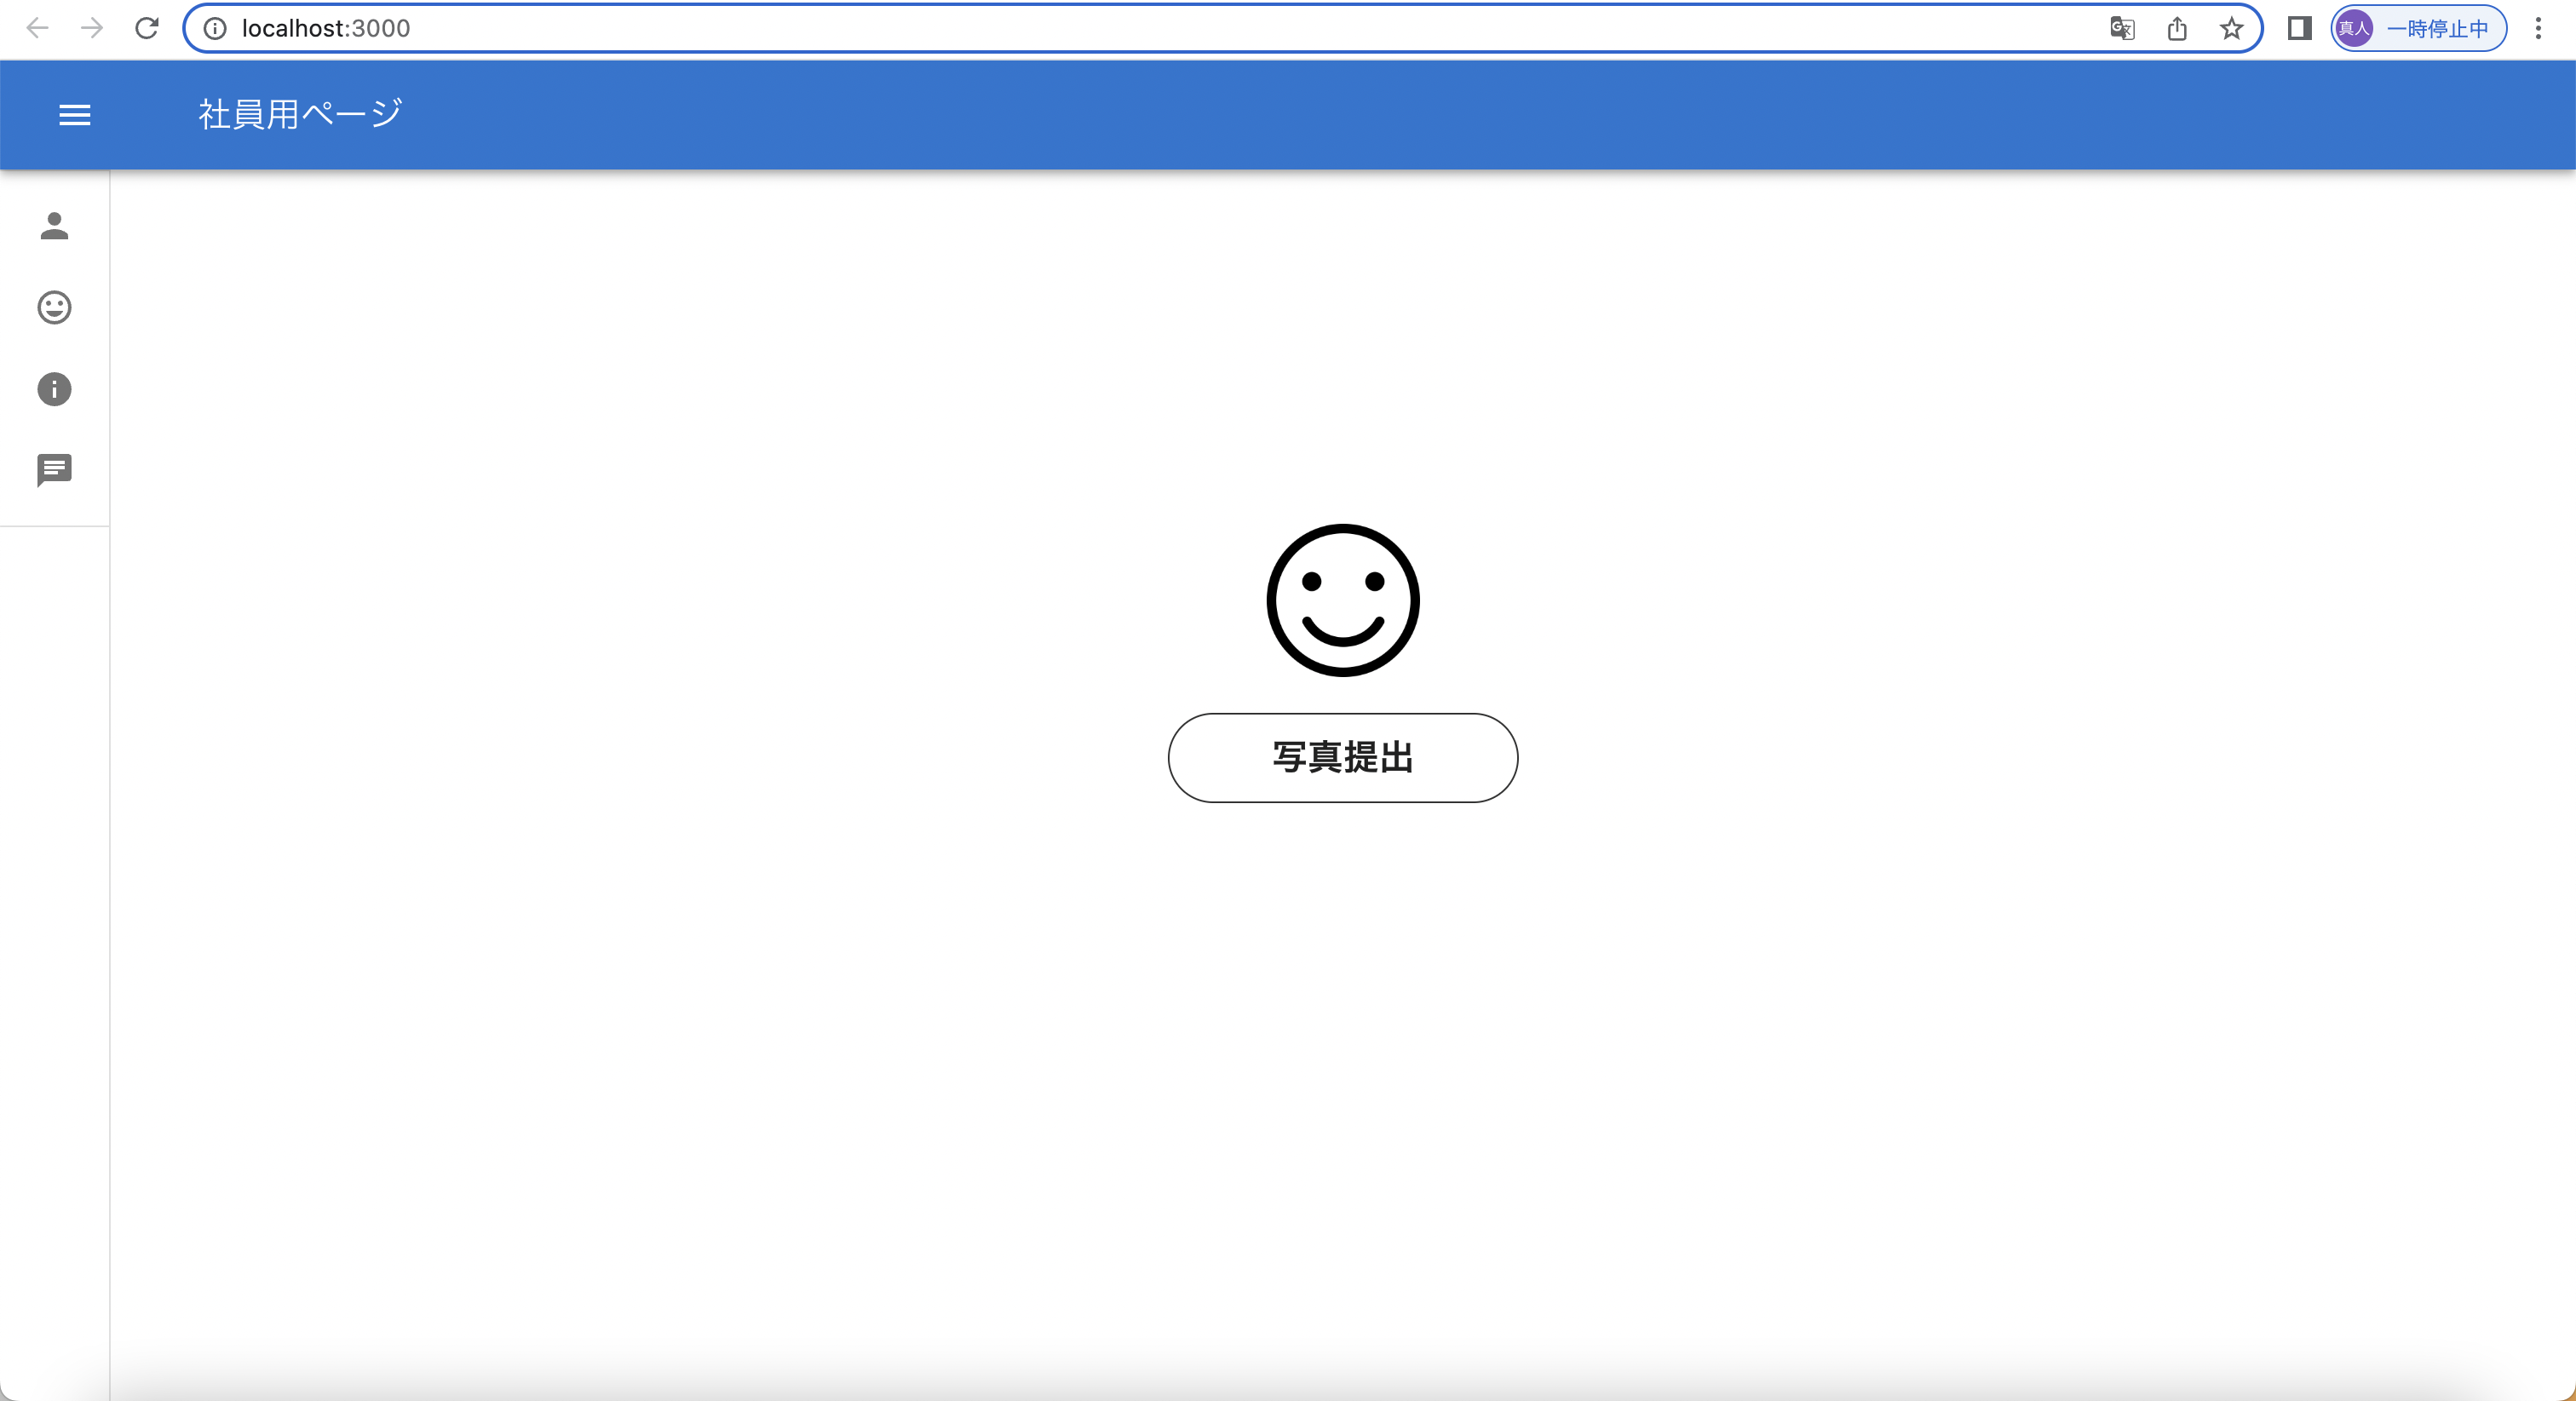
\includegraphics[scale=0.3, clip]{./img/sample1.png}
			\caption{提出画面}
			\label{fig:図の名前}
	\end{center}
\end{figure}

\begin{figure}[!h]
	\begin{center}
			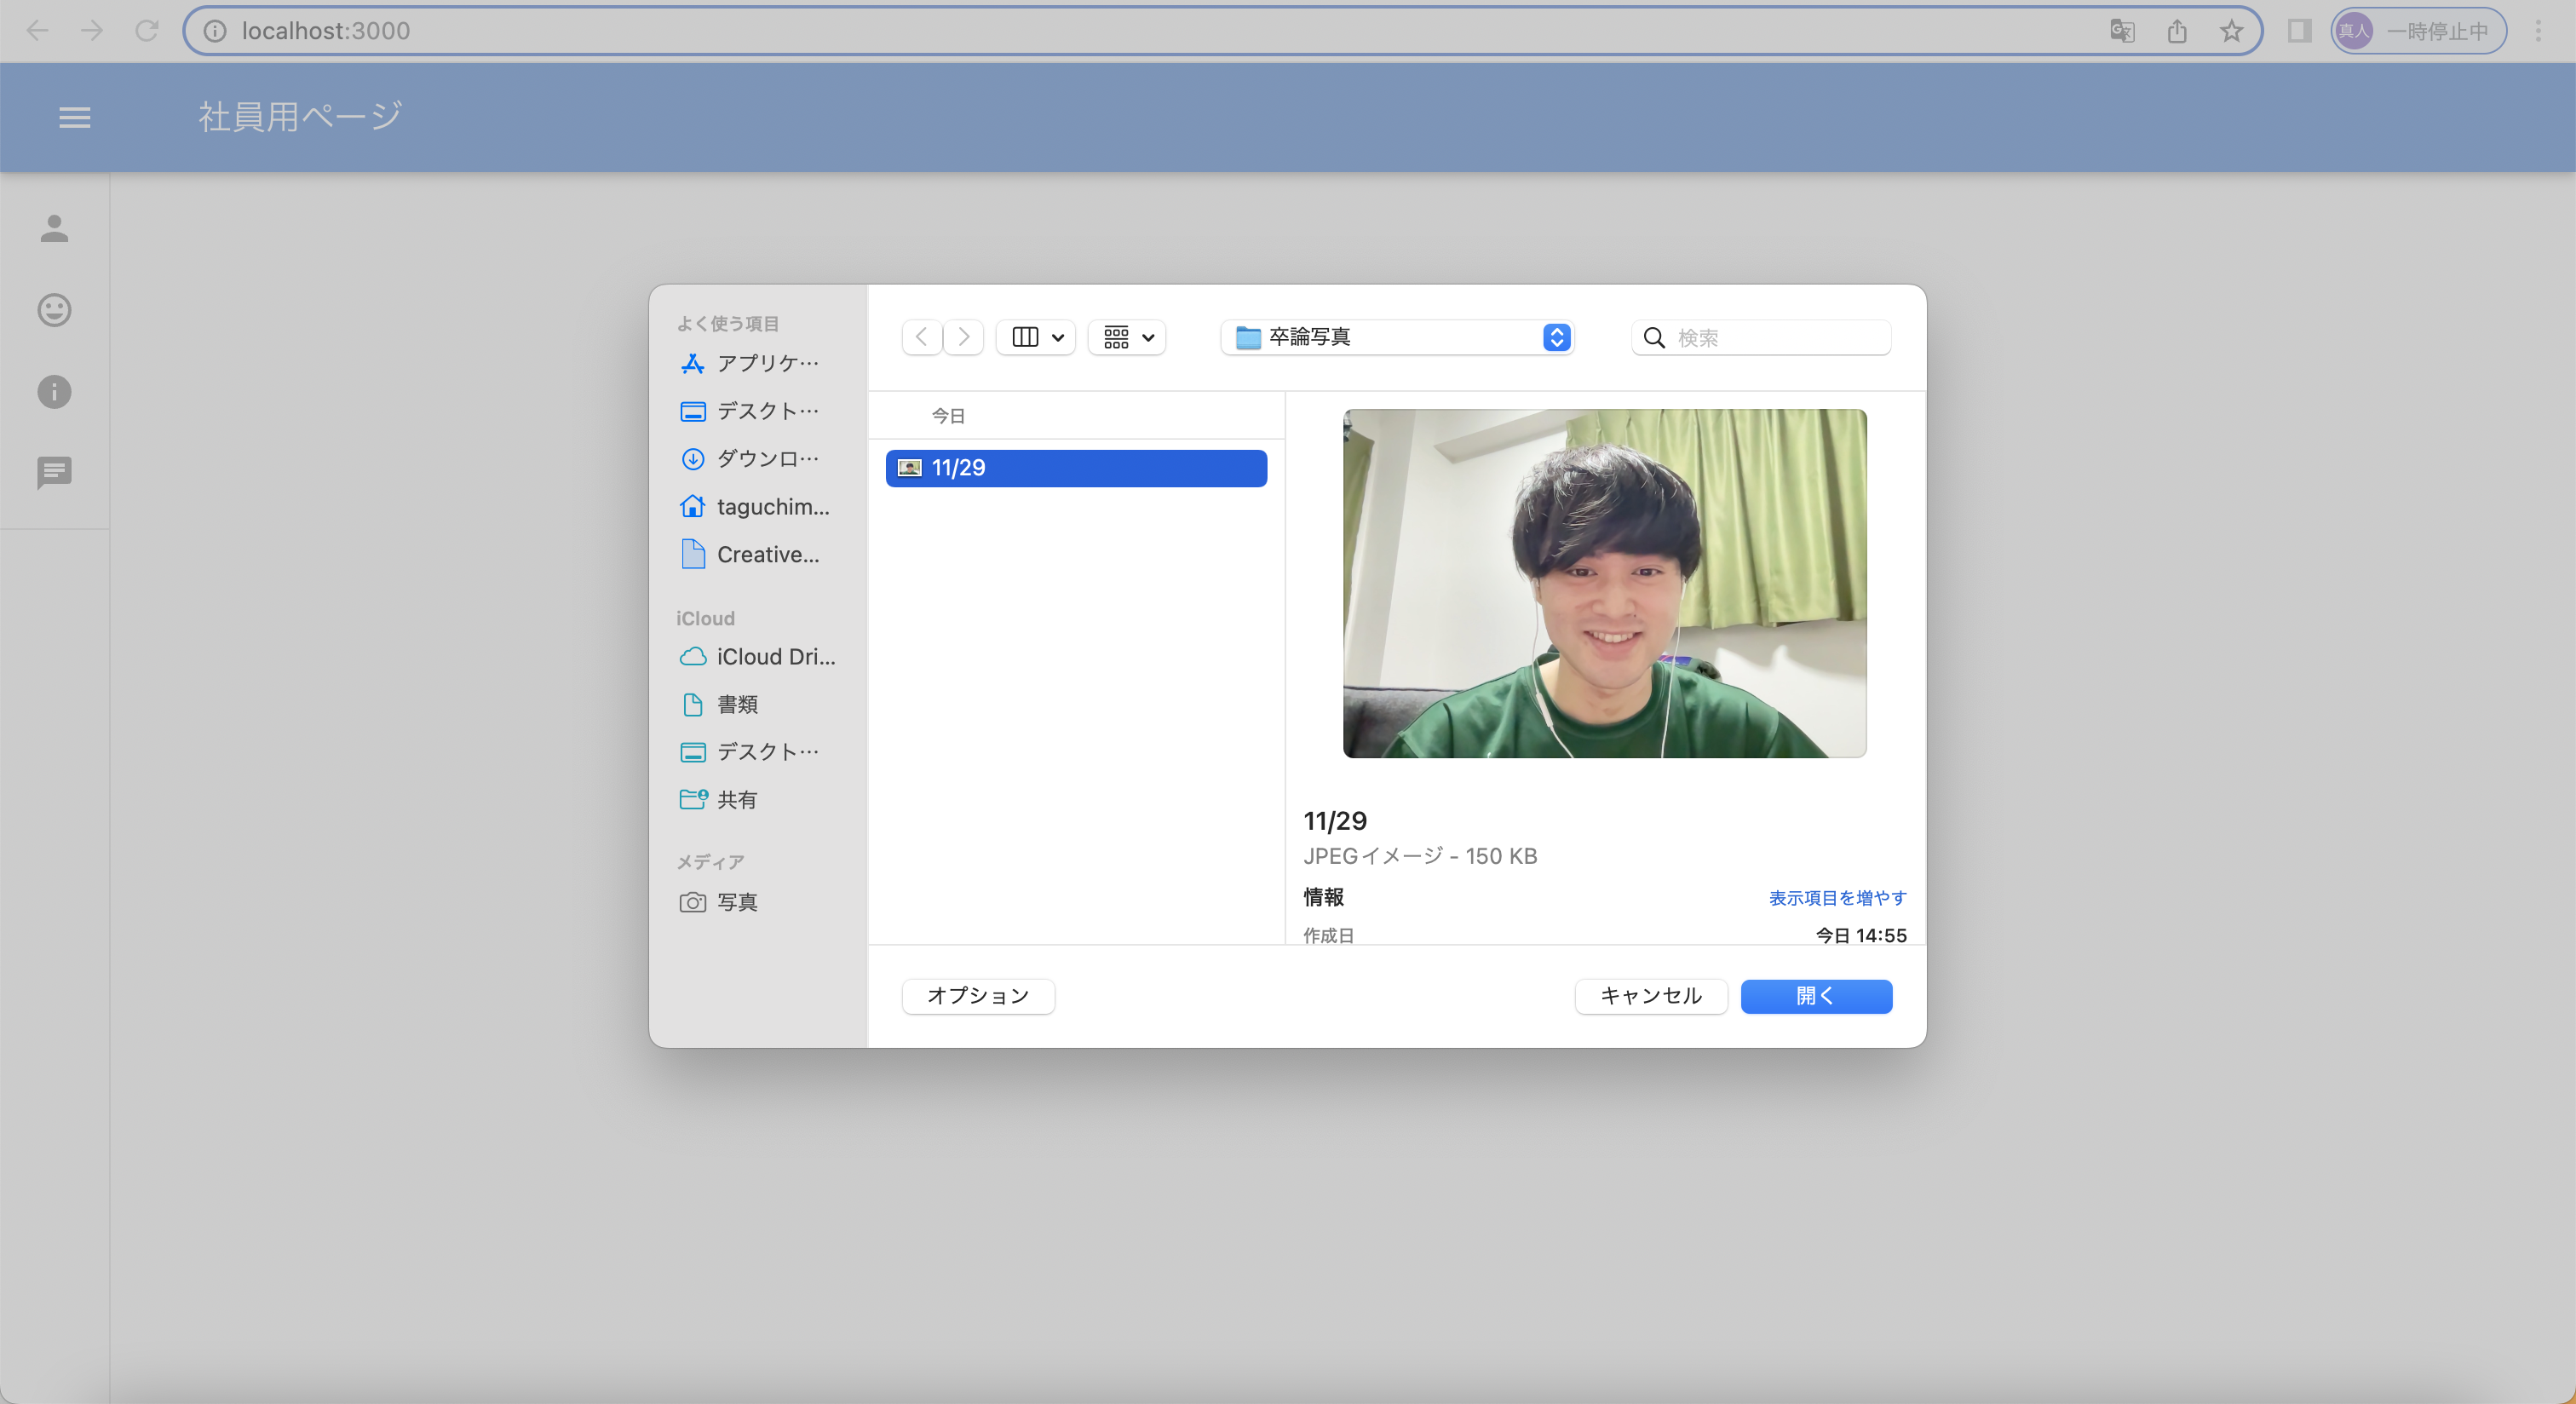
\includegraphics[scale=0.3, clip]{./img/sample2.png}
			\caption{写真選択画面}
			\label{fig:図の名前}
	\end{center}
\end{figure}

\begin{figure}[!h]
	\begin{center}
			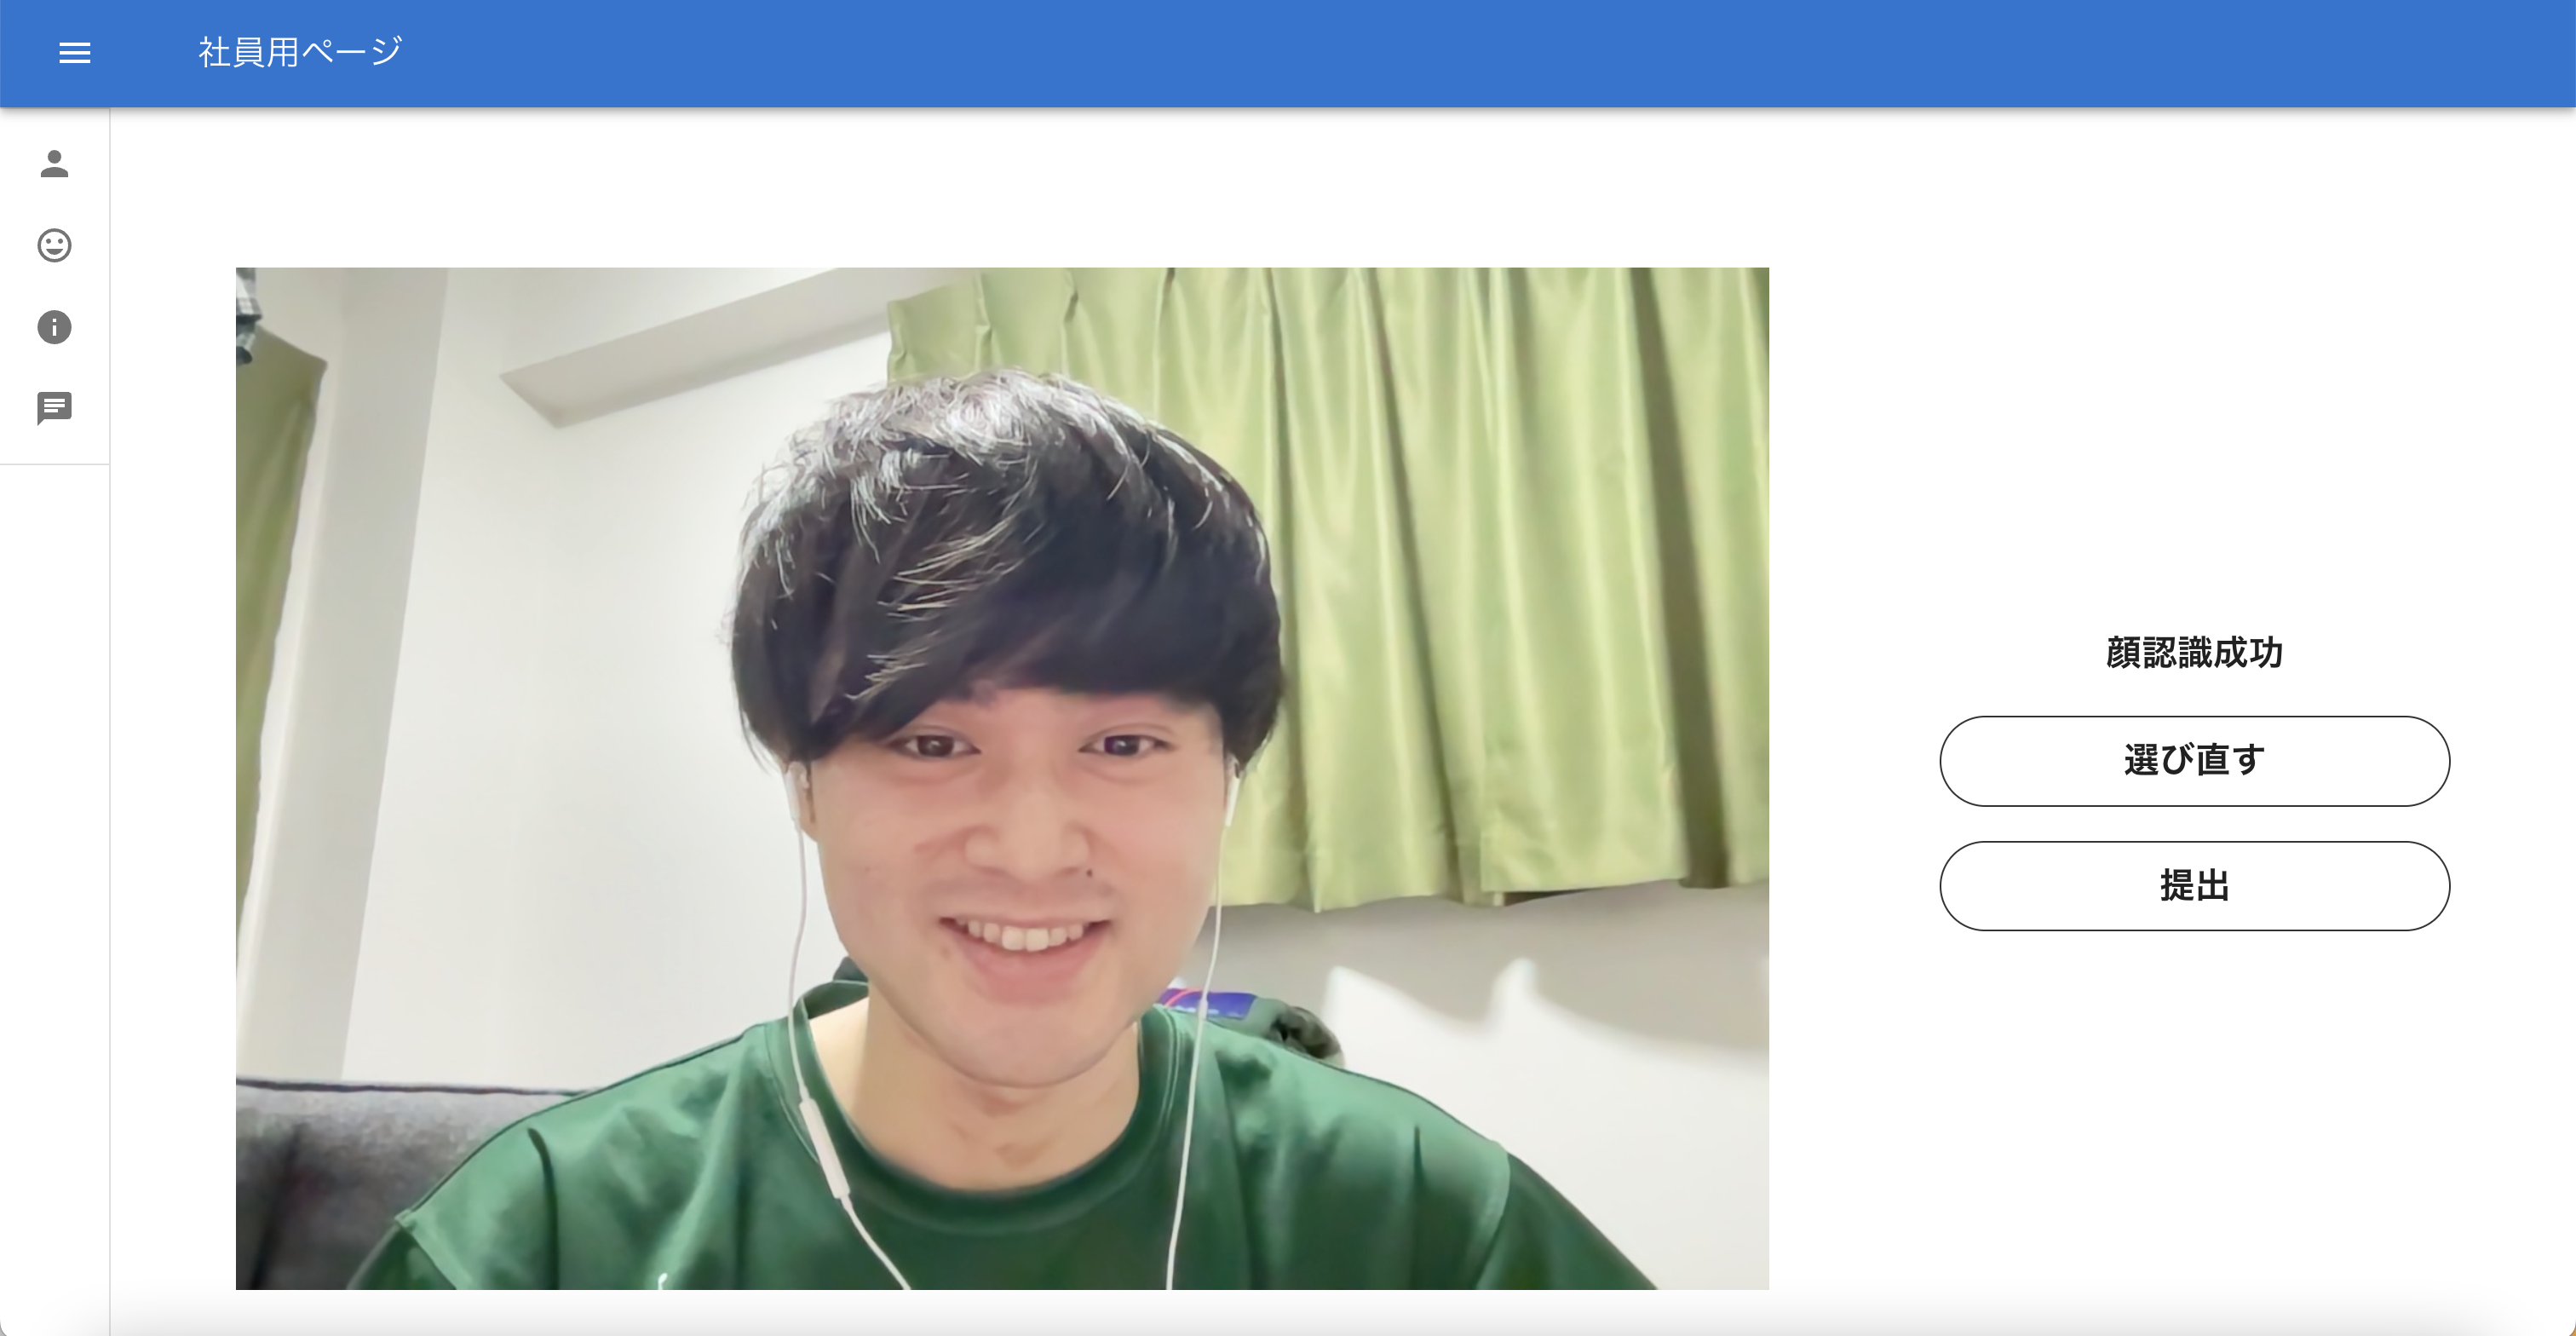
\includegraphics[scale=0.3, clip]{./img/sample3.png}
			\caption{画面}
			\label{fig:図の名前}
	\end{center}
\end{figure}

\begin{figure}[!h]
	\begin{center}
			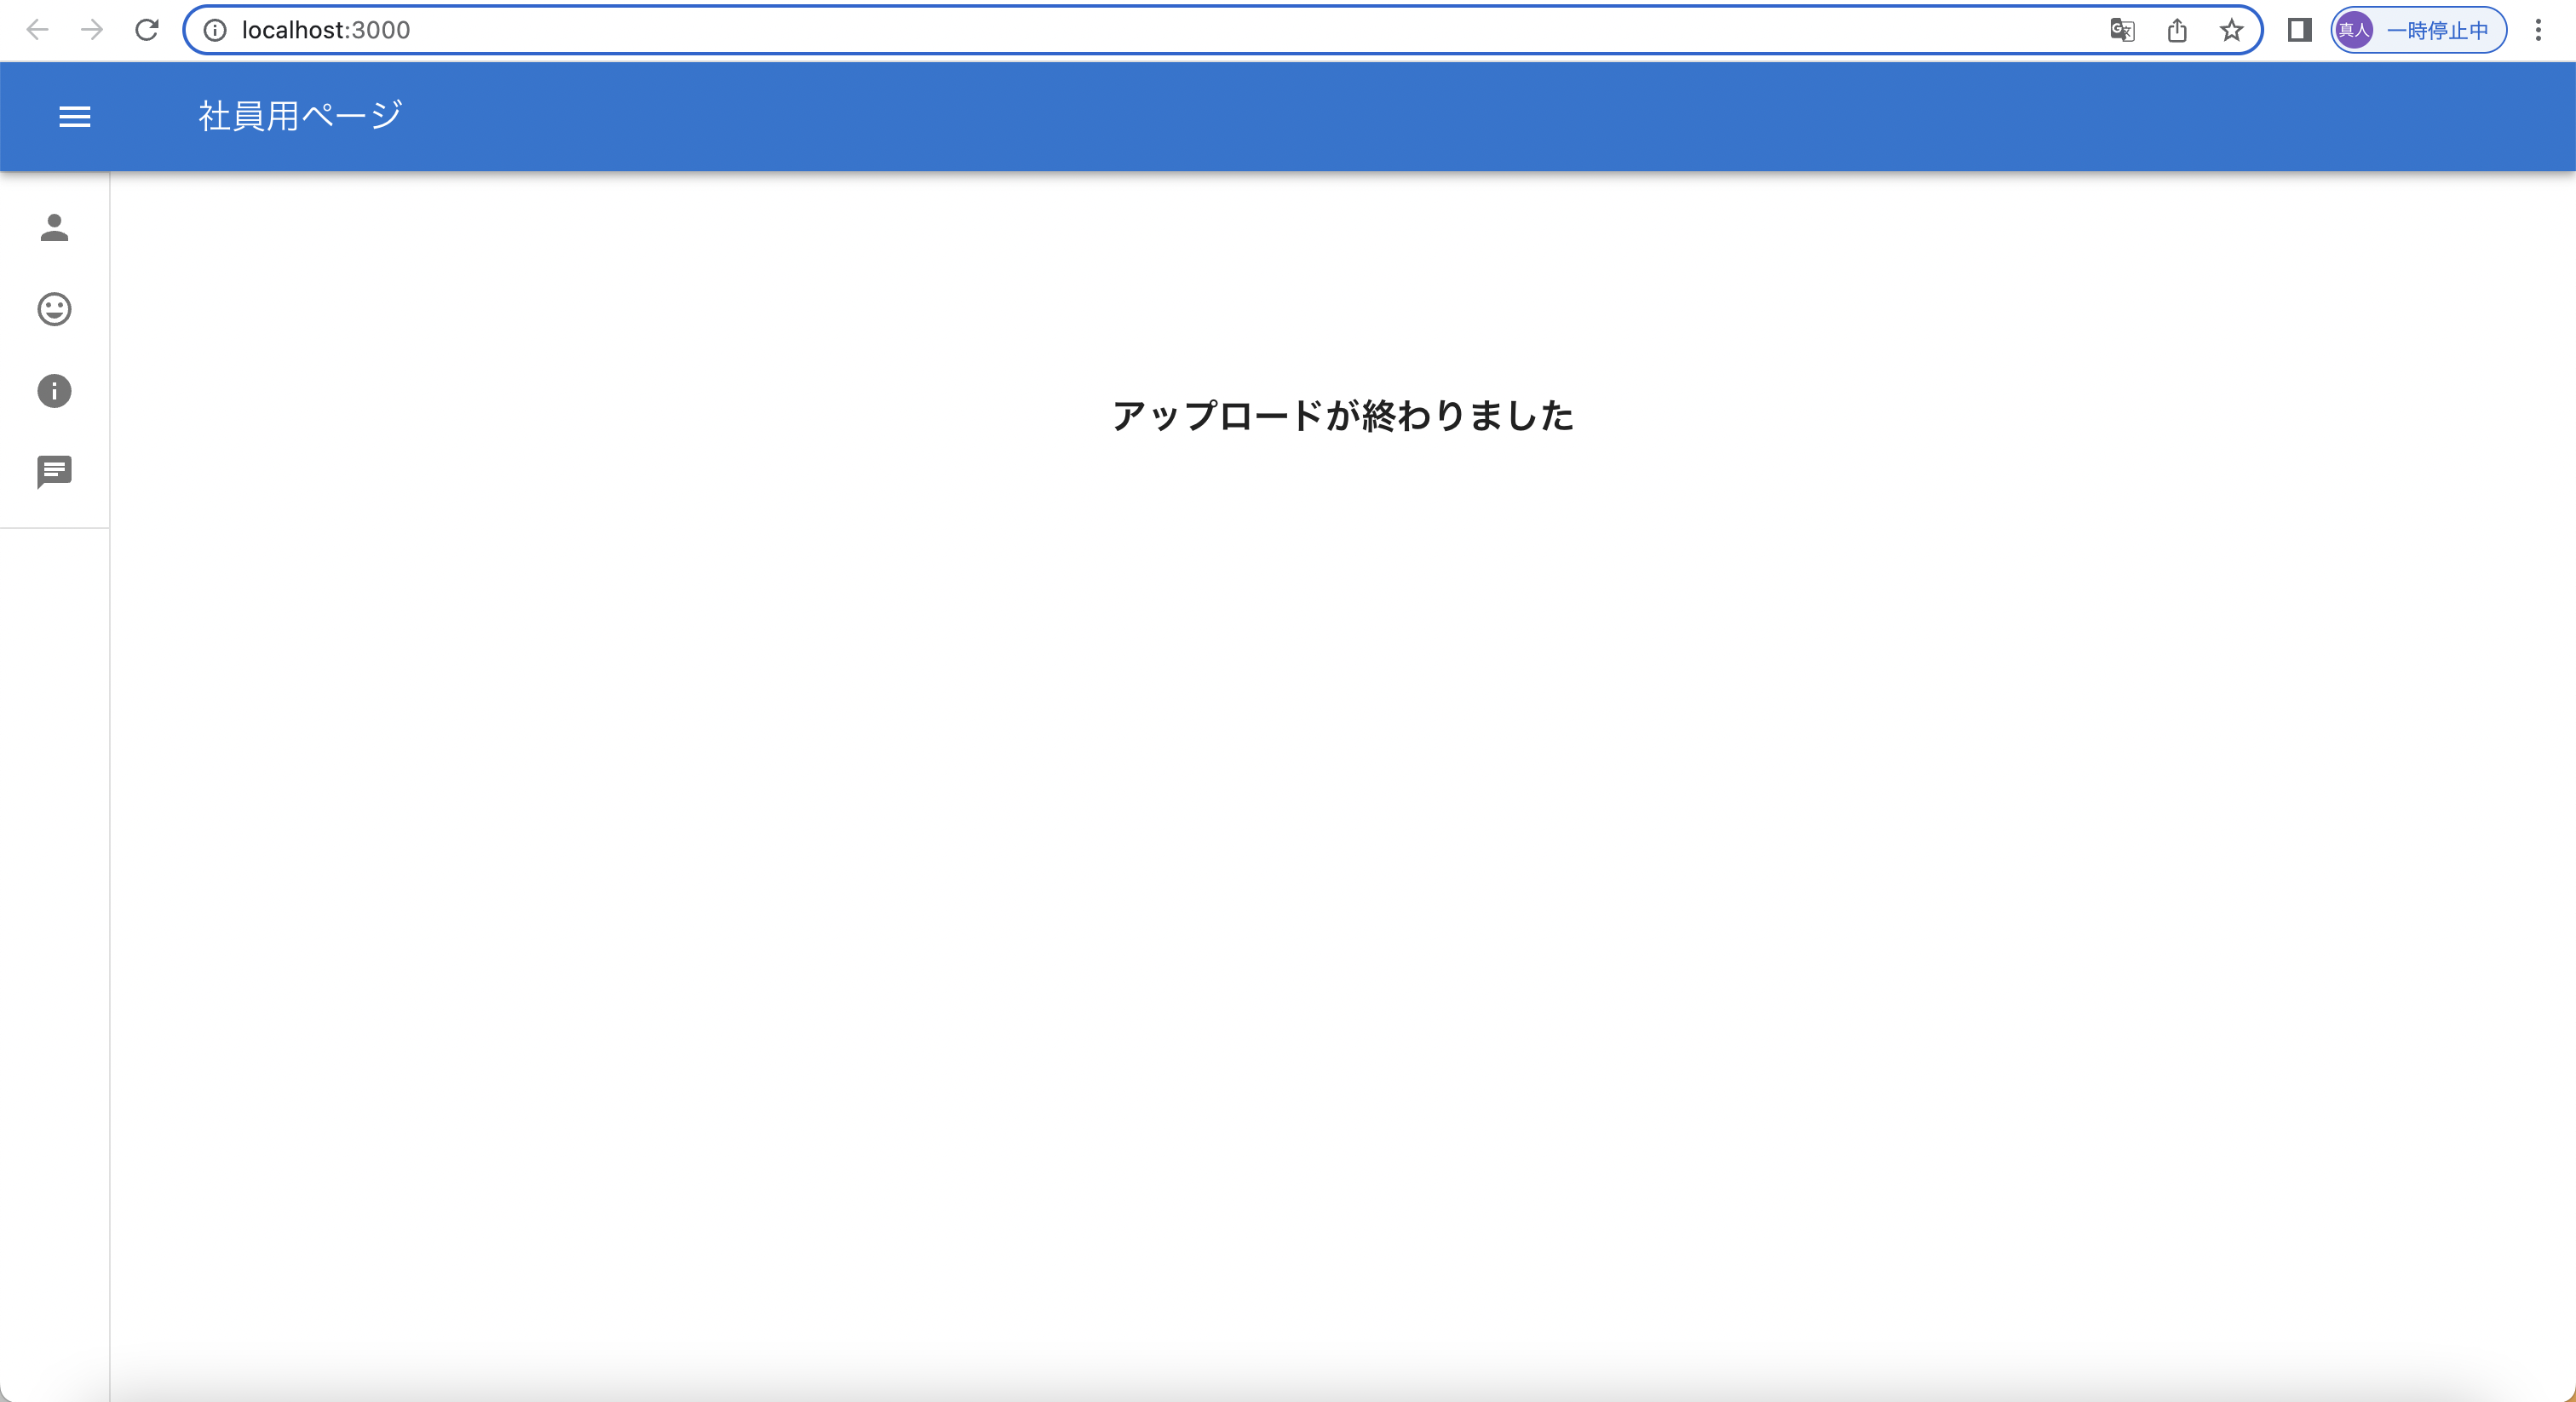
\includegraphics[scale=0.3, clip]{./img/sample4.png}
			\caption{提出完了画面}
			\label{fig:図の名前}
	\end{center}
\end{figure}

\clearpage

\begin{figure}[!h]
	\begin{center}
			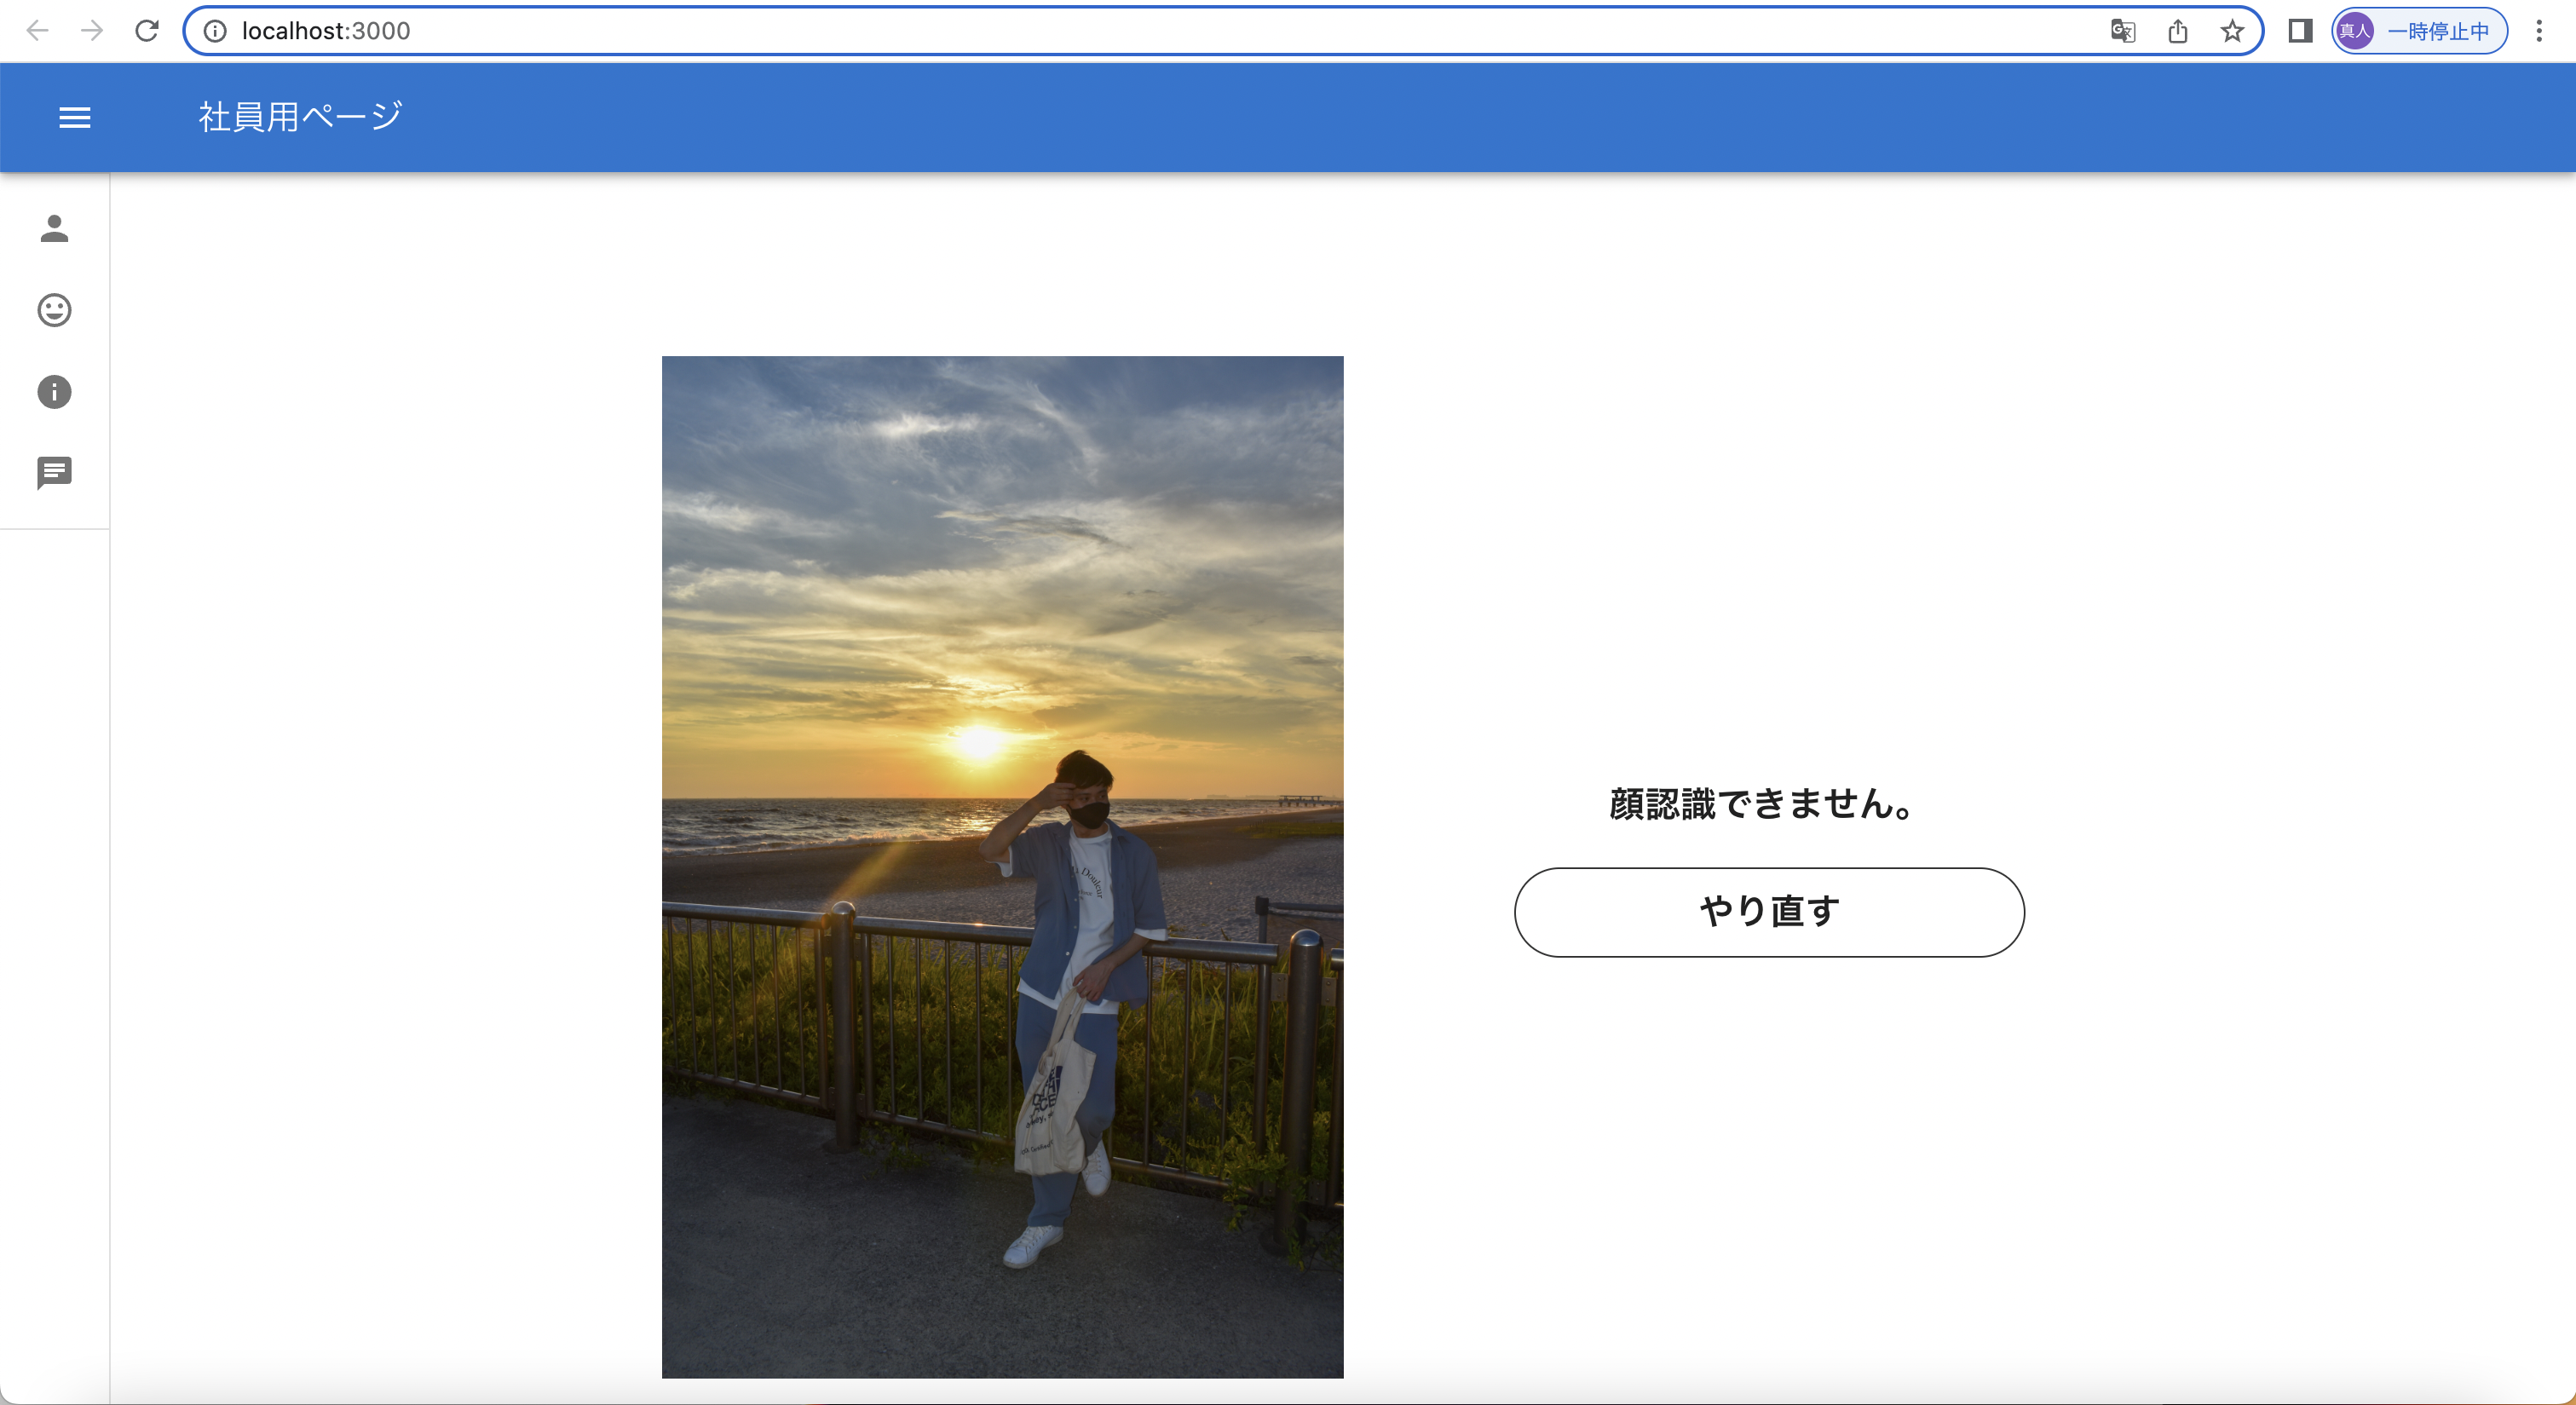
\includegraphics[scale=0.3, clip]{./img/sample5.png}
			\caption{顔認識失敗画面}
			\label{fig:図の名前}
	\end{center}
\end{figure}

\section{管理者の社員管理機能}

\section{掲示板機能}

\section{チャット機能}